% SPDX-License-Identifier: CC-BY-SA-4.0
% Copyright (c) 2026 Luis Alonso
%
% This file is part of luis_alonso/Notas-Japones.
%
% Licensed under Creative Commons Attribution-ShareAlike 4.0 International (CC BY-SA 4.0).
% You may share and adapt this material for any purpose,
% as long as you provide attribution and distribute adaptations under the same license.
%
% License: https://creativecommons.org/licenses/by-sa/4.0/
% Source:  https://git.lalonso.com/luis_alonso/Notas-Japones
%
% Note: Third-party content (if any) is excluded from this license and is marked where used.

\documentclass[a4paper,lualatex,ja=standard,base=10pt]{bxjsarticle}
\usepackage{setup}
\usepackage{ulem}

\newcommand{\m}[1]{\textcolor{blue}{#1}}
\newcommand{\rmv}[1]{\textcolor{red}{\sout{#1}}}
\newcommand{\masuToJisho}[3]{#1\textcolor{blue}{#2}\textcolor{red}{\sout{ます}} & #1\textcolor{blue}{#3}}

\title{\ruby{第|０１|課}{だい||か} LV4}
\author{アロンゾ　ルイス}

\begin{document}
\setcounter{page}{1}

\maketitle{}
\thispagestyle{fancy}

\section{新しいことば \ruby{趣|味}{しゅ|み}}
\medskip

\textbf{Actividades}

\begin{itemize}
  \item \ruby{料|理}{りょう|り} (Cocinar)
  \item \ruby{お|菓|子}{|か|し} (Dulces)
  \item \ruby{演|劇}{えん|げき} (Teatro)
  \item \ruby{切|手}{きっ|て}を\ruby{集}{あつ}めます (Coleccionar)
  \item \ruby{将|棋}{しょう|ぎ} (Shogi ajedrez japones)
  \item \ruby{凧|揚|げ}{たこ|あ|げ} (Volar cometas)
  \item \ruby{囲|碁}{い|ご} (Go, juego)
  \item \ruby{編|み|物}{あ||もの} (Tejer)
  \item ガーデニング (Jardinería)
  \item サイクリング (Ciclismo)
  \item \ruby{水|泳}{すい|えい} (Natación)
  \item \ruby{乗|馬}{じょう|ば} (Equitación)
\end{itemize}

\section{Forma \ruby{辞|書}{じ|しょ}}

Forma diccionario.

Tambien se usa para describir acciones recurrentes como pasatiempos:

\begin{itemize}
  \item ビデオゲームをすることです。
  \item 本を読むことです。
\end{itemize}


\subsection{１グループ Verbos que terminan en sonido イます}

Para transformar los verbos se pasa el sonido de イ a su equivalente en ウ.

\begin{itemize}
  \item い pasa a う
  \item き pasa a く
  \item し pasa a す
  \item ち pasa a つ
  \item に pasa a ぬ
  \item ひ pasa a ふ
  \item み pasa a む
  \item り pasa a る
\end{itemize}

\begin{VocabTable}[0.15\linewidth][→][P,P]
  \masuToJisho{つく}            {り} {る}\\
  \masuToJisho{\ruby{行}{い}}   {き} {く}\\
  \masuToJisho{\ruby{言}{い}}   {い} {う}\\
  \masuToJisho{\ruby{泳}{およ}} {ぎ} {ぐ}\\
  \masuToJisho{\ruby{話}{はな}} {し} {す}\\
  \masuToJisho{\ruby{持}{も}}   {ち} {つ}\\
  \masuToJisho{\ruby{死}{し}}   {に} {ぬ}\\
  \masuToJisho{\ruby{遊}{あそ}} {び} {ぶ}\\
\end{VocabTable}

\subsection{２グループ Verbos que terminan en sonido エます y que tienen exactamente tres caracteres}

Para transformar los verbos de este grupo se quita la parte del ます y se cambia por る.

Por ejemplo:

\begin{itemize}
  \item 食べ\textcolor{red}{\sout{ます}} pasa a 食べ\textcolor{blue}{る}
  \item 見\textcolor{red}{\sout{ます}} pasa a 見\textcolor{blue}{る}
\end{itemize}

Hay casos excepcionales como:

\begin{itemize}
  \item できます pasa a できる
  \item \ruby{浴}{あ}びます pasa a \ruby{浴}{あ}びる
  \item \ruby{起}{お}きます pasa a \ruby{起}{お}きる
  \item \ruby{借}{か}ります pasa a \ruby{借}{か}りる
\end{itemize}

\begin{VocabTable}[0.15\linewidth][→][P,P]
  \masuToJisho{\ruby{上}{あ}}   {げ} {げる}\\
  \masuToJisho{で}              {き} {きる}\\
  \masuToJisho{\ruby{起}{お}}   {き} {きる}\\
  \masuToJisho{\ruby{集}{あつ}} {め} {める}\\
  \masuToJisho{い}              {} {る}\\
  \masuToJisho{\ruby{来}{き}}   {} {る}\\
\end{VocabTable}

\subsection{３グループ Verbos します/来ます y SUST＋します}

Son verbos especiales y sustantivos convertidos en verbos.
Para transformar a esta forma se remueve el ます y se agrega する.

\begin{VocabTable}[0.15\linewidth][→][P,P]
  \textcolor{red}{\sout{します}} & \textcolor{blue}{する}\\
  \ruby{来}{き}\textcolor{red}{\sout{ます}} & \textcolor{blue}{\ruby{来}{く}る}\\
  \ruby{勉強}{べんきょう}\textcolor{red}{\sout{します}} & \ruby{勉強}{べんきょう}\textcolor{blue}{する}\\
  \ruby{運動}{うんどう}\textcolor{red}{\sout{します}} & \ruby{運動}{うんどう}\textcolor{blue}{する}\\
  \ruby{掃除}{そうじ}\textcolor{red}{\sout{します}} & \ruby{掃除}{そうじ}\textcolor{blue}{する}\\
  \ruby{運転}{うんてん}\textcolor{red}{\sout{します}} & \ruby{運転}{うんてん}\textcolor{blue}{する}\\
\end{VocabTable}

\section{Oraciones con \ruby{時}{とき}}

Oraciones para indicar que se hace/hizo en un tiempo en concreto aunque puede no ser especifico.

\begin{figure}[H]
  \centering
  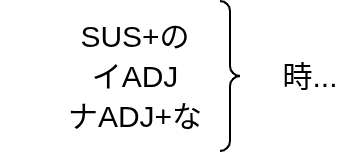
\includegraphics[width=0.4\linewidth]{assets/toki.png}
  \caption{Formar oraciones con 時}
\end{figure}

Ejemplos:

\begin{itemize}
  \item \ruby{暇}{ひま}な\ruby{時}{とき}、\ruby{料理}{りょうり}を\ruby{作}{つく}ります。
  \item \ruby{子}{こ}どもの\ruby{時}{とき}、\ruby{運動}{うんどう}よく\ruby{遊}{あそ}びました。
  \item \ruby{寒}{さむ}い\ruby{時}{とき}、コーヒーを飲みます。
\end{itemize}

\end{document}

